\section{Introduction}

\label{2302:sec:intro}
A detailed understanding of the performance of stochastic gradient descent (SGD) in neural networks is a major endeavor in machine learning, and  significant progress was achieved in the context of large two-layer neural networks. In particular the optimization over wide two-layer neural networks can be rigorously studied using a well-defined partial differential equation (PDE) \citep{mei2018mean,chizat2018global,rotskoff2022trainability,sirignano2020mean}. A consequence of these results is the global convergence of overparametrized two-layer networks towards perfect learning provided that the number of hidden neurons is large, the learning rate is sufficiently small, and enough data is at disposal. This line of work is commonly referred to as the \emph{mean-field limit} of neural networks. The phenomenology in this regime was also studied for synthetic data with simple target functions by \cite{mei2019mean,abbe2022merged}.

Interestingly, the SGD dynamics of two-layer neural networks trained on synthetic Gaussian data was considered as early as in the seminal work of \cite{saad1995line,saad1995exact,saad1996dynamics}, and has witnessed a renewal of activity over the last few years \citep{vershynin2018high,goldt2019dynamics,veiga2022phase,arous2022high}. However, differently from the mean-field limit, these works investigated the opposite limit of \emph{fixed} hidden layer width and \emph{diverging} data dimension, and studied the limiting SGD dynamics through a set of ordinary differential equations (ODEs).

Given these different limits, one may naturally wonder what is the relation, if any, between these sets of works. More generally, given data in dimension $d$ and a two-layer network with $p$ hidden units trained by SGD with a learning rate $\gamma$, one might inquire about the different regimes beside the mean-field ($p \to \infty$) and high-dimensional ($d \to \infty$) ones. This is the question investigated in this work. We consider a two-layer network trained on Gaussian data and labels given by a similar, though not necessarily identical, two-layer neural network target (hereafter also referred to as the \emph{teacher}), and investigate the one-pass stochastic gradient descent (SGD) dynamics as a function of the relevant parameters $d,p$ and $\gamma$. As summarized in Fig.\ref{2302:fig:triangle}, we show that as long as $\sfrac{\gamma}{dp} \to 0^+$, a unifying deterministic description can be provided. In particular, our description recovers all the previously studied limits (mean field, high-dimensional and the classical gradient flow regime) and builds a bridge between them in a unified formalism. Namely, our \textbf{main contributions} are:
\begin{itemize}
    \item Starting from the general approach of \cite{saad1995line,saad1996dynamics}, we build on the non-asymptotic results \cite{veiga2022phase} and show how it allows to describe the entire phase space in Fig. \ref{2302:fig:triangle}, that interpolates between the high-dimensional, classical, and mean-field limits.
     \item We unveil a remarkable dimension independence  in the classical gradient-flow limit: once the initial conditions are given, the dynamics in terms of the sufficient statistics turns out to be {\it entirely} independent of the data dimension $d$.
     \item We explicitly construct the mean-field solution starting from the ODEs in the mean-field regime, bridging the hitherto different worlds of \citep{saad1995line,saad1996dynamics} with the mean-field "hydrodynamic" approach. More precisely, for $p \to \infty$, we show how the ODEs simplify and give rise to a mean-field PDE, thanks to a decoupling of the learning dynamics that is found to remain close to a low-dimensional subspace spanned by the target principal directions.
    \item We further discuss how the SGD dynamics in the mean-field regime behave differently whether the input dimension $d$ is small or large, leading to different finite-$d$ and high-$d$ dimensionless PDEs. This generalizes the recent ``dimension-free'' results in \cite{hajjar2023symmetries,abbe2022merged}.
    \item We provide a numerical solver for these equations. A GitHub repository with the code employed in the present work is available  on \href{https://github.com/IdePHICS/DimensionlessDynamicsSGD}{GitHub repository}.  Additionally, we discuss the interesting case of quadratic activation that allows to drastically reduce the complexity of the ODEs \& PDEs.
\end{itemize}

\begin{figure}
  \begin{center}
    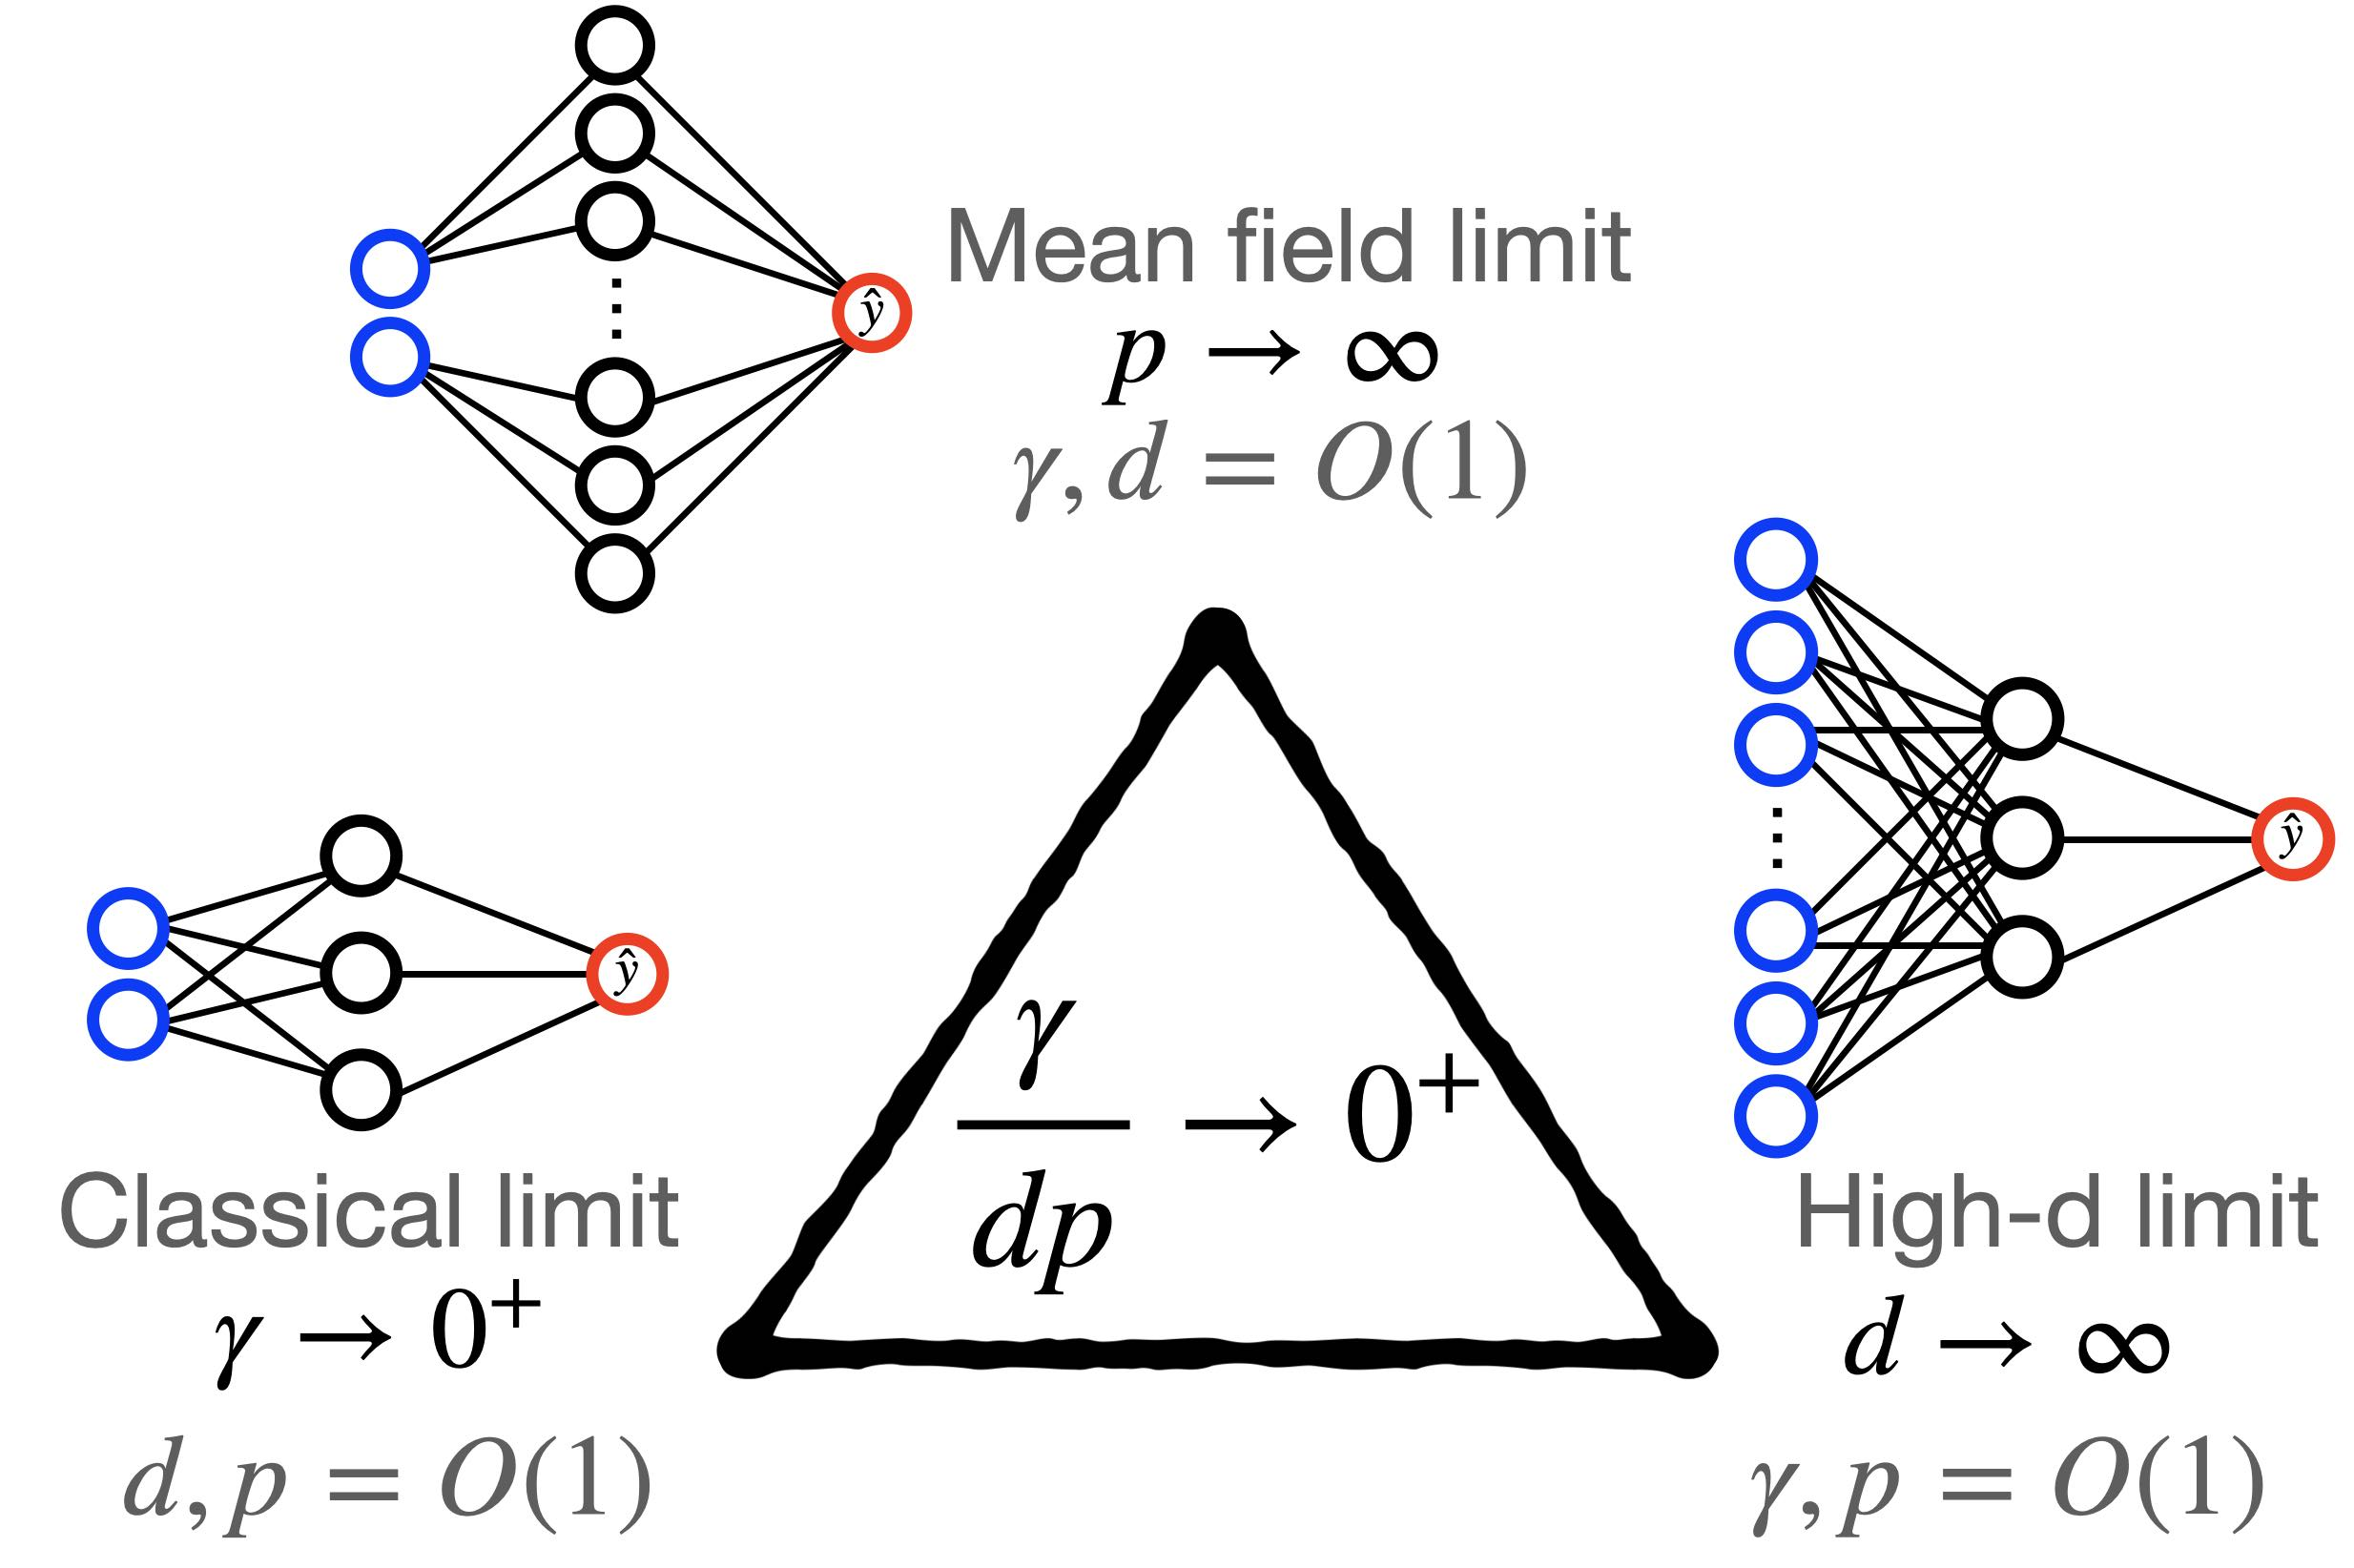
\includegraphics[height=0.49\textwidth]{figs/TriangleV3}
  \end{center}
 \caption{We discuss a unifying low-dimensional description of the one-pass SGD dynamics Equation~\eqref{2302:eq:def:sgd} for two-layers neural networks as $\sfrac{\gamma}{dp} \to 0^+$. This includes, in particular, the mean-field ($p \to \infty$), the high-dimensional ($d \to \infty$) and the classical gradient flow ($\gamma \to 0$) limits.}
\label{2302:fig:triangle}
\end{figure}
\paragraph{Related work ---} Stochastic gradient descent was first introduced \cite{robbins1951stochastic} as a stochastic approximation method, and later applied as an approximation to population risk minimization in \cite{bottou2003large,bottou2007tradeoffs}. Its properties have been extensively studied for finite learning rate and input dimension in the strongly convex setting \citep{pflug1986stochastic,moulines2011non,dieuleveut2017harder,dieuleveut2020bridging}, and more recently in convex problems in the interpolating regime \citep{ma2018power,vaswani2019fast,zou2021benign,varre2021last}, to cite a few.   High-dimensional limits of SGD were studied in \cite{vershynin2018high,arous2021online} for non-convex, single-index models. Recently, \cite{arous2022high} has generalized and abstracted this discussion.
    
In the context of two-layer neural networks, the high-dimensional limit of SGD draws back from the seminal work of \cite{saad1995line,saad1995exact,saad1996dynamics} and was subsequently studied by many authors  under different settings \citep{biehl1995learning,copelli1995line,biehl1996transient,goldt2019dynamics,goldt2020modeling,goldt2022gaussian,refinetti2021classifying}. The infinite-width (a.k.a. mean-field) limit of the SGD dynamics of two-layer neural networks was studied by \cite{mei2018mean,chizat2018global,rotskoff2022trainability,sirignano2020mean}, who proved global convergence under certain conditions on the architecture and initialization. A bridge between these two limits was discussed by \cite{veiga2022phase}, who studied the joint limit where the hidden-layer width and the learning rate scale with the diverging input dimension. 

Closer to us, dimension-free limits of the mean-field equations have been derived by \cite{abbe2022merged} for low-dimensional target functions in the hypercube and by \cite{hajjar2023symmetries} for ReLU networks when the target is invariant under certain symmetries. \cite{boursier2022gradient} has proven global convergence of the gradient flow dynamics at finite width for orthogonal input data. 
%%%%%%%%%%%%%%%%%%%%%%%%%%%%%%%%%%%%%%%%%%%%%%%%%%%%%%%%%%%%%%%%%%%%%%%%%%%%%%
